\fancyhead[LO, RE]{Conclusion}

\paragraph{} L'alignement\index{Alignement} est un procédé encore en développement qui peut prendre plusieurs formes et se baser sur des textes variés. Il peut être nécessaire de trouver une méthode propre pour l'effectuer, selon nos besoins, ce que nous avons finalement accompli. Au fur et à mesure du stage, nous avons procédé à de nombreuses opérations afin de travailler le texte et d'en ressortir divers éléments et données. Cela nous a permis principalement de mettre en place une démarche afin d'accomplir l'objectif du stage~: un alignement partiel\index{Alignement!alignement partiel}, ciblé\index{Alignement!alignement cible@alignement ciblé} à partir d'un lexique juridique. Nous avons donc maintenant à notre disposition un processus, partant d'un manuscrit numérisé, forme de base de notre corpus, et arrivant à un tableau d'alignement\index{Alignement!tableau d'alignement}, simple ou avancé, finalité de notre stage, qui peut être représenté à l'aide du schéma suivant.
\begin{figure}[H]
    \centering
    \fbox{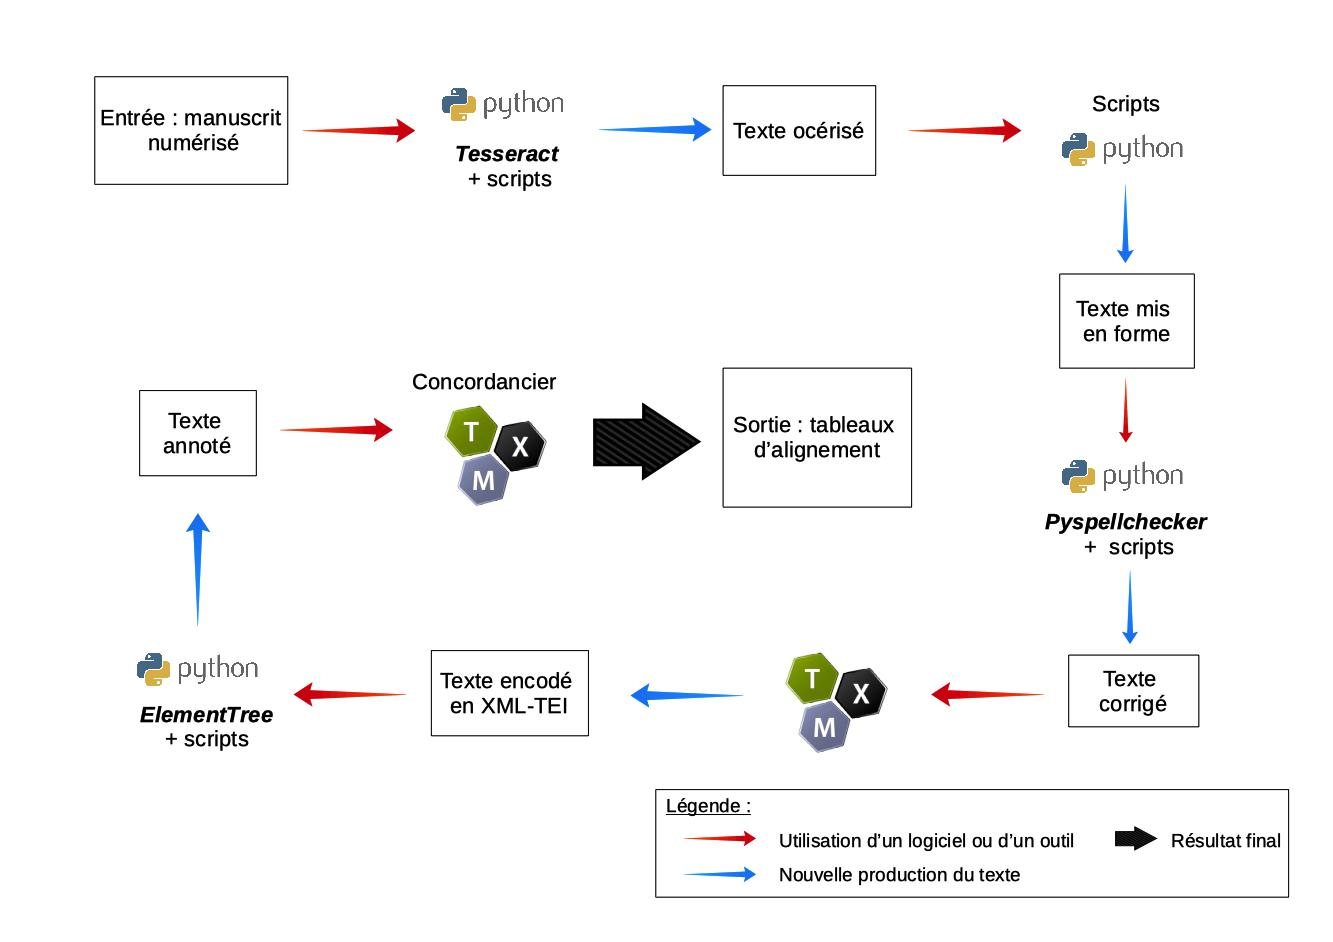
\includegraphics[width=16cm]{Conclusion/processus_pour_alignement.jpg}}
    \caption{Processus représentant la démarche pour effectuer l'alignement\index{Alignement}}
    \label{fig:processus_alignement}
\end{figure}
Nous partons ainsi de notre fichier de base et à chaque utilisation d'un nouveau logiciel, d'un nouvel outil et/ou de l'exécution d'un script Python, nous obtenons une nouvelle forme du texte, texte qui évolue progressivement, afin d'atteindre une forme qui, à l'aide du concordancier\index{Concordancier} de \textsc{txm}, nous permet de rédiger les tableaux d'alignement\index{Alignement!tableau d'alignement}. Nous avons donc un processus ne nécessitant pas une grande quantité d'étapes, impliquant l'installation de quelques logiciels et l'exécution de plusieurs scripts pour produire à la fin un alignement\index{Alignement} devant reposer sur un lexique. 

\paragraph{} Nous avons effectué, en parallèle de notre démarche principale, d'autres opérations sur notre corpus. Certaines de ces opérations étaient requises car elles permettaient de répondre à un des enjeux du stage. Grâce aux analyses textuelles, par la lecture et par quelques outils, nous avons pu établir la généalogie des éditions à disposition. Cette finalité nous a ainsi permis d'obtenir diverses informations sur les éditions en elle-même et non juste sur un chapitre en particulier. Cela a, de plus, aidé au travail futur et à la démarche principale puisque cela a fourni une base de connaissances sur les origines de chacune des éditions. D'autres opérations n'étaient pas obligatoires mais donnaient la possibilité d'approfondir nos connaissances sur le texte, de manière plus générale que l'alignement ciblé\index{Alignement!alignement cible@alignement ciblé} que nous avons effectué et moins limitée par le travail exclusif d'un seul chapitre. Grâce aux statistiques textuelles\index{Statistique textuelle} que nous avons extraites des différents chapitres traités, nous avons pu en apprendre plus sur le lexique, sur la formation des textes, sur leur structure mais aussi sur leurs différences et sur ce qui fait leur particularité. Ces analyses ont offert un point de vue plus général sur les textes que le seul travail basé sur l'aspect juridique qui a conduit à l'alignement\index{Alignement}. Ces opérations parallèles nous ont donc apporté des informations supplémentaires et intéressantes sur notre corpus, sans avoir à être liées exclusivement à l'alignement\index{Alignement}.

\paragraph{} Tout le travail n'a tout de même pas été fait. Si la démarche a commencé à être effectuée avec les éditions allemandes, cela ne représente qu'une petite fraction du travail et l'alignement\index{Alignement} lui-même, élément majeur du projet, n'aura pas été du tout réalisé pour l'allemand, pourtant une des premières langues dans laquelle le corpus a été traduit. Les textes n'ont pas été corrigés, ni importés sur le logiciel et il n'a pas été possible de retravailler la liste de termes juridiques pour rajouter les bons termes en allemand. Sans cela, il n'était pas possible de compléter le travail et cela restera donc une partie importante qui demeure inachevée. Par ailleurs, vers la fin du stage, de nouvelles éditions en français, allemand et italien ont été acquises, soit car il a enfin été possible de les numériser, soit car elles n'ont été découvertes qu'à ce moment, et le temps imparti pendant le stage empêchait de réaliser toute la démarche et de rajouter ces textes dans les analyses effectuées et dans les tableaux d'alignement\index{Alignement!tableau d'alignement}. Cela représente donc à la fois un travail inachevé puisque le corpus était à disposition et une perspective de travail pour la suite.

\paragraph{} Nous avons réalisé notre travail efficacement et sans trop de difficultés mais il s'est tout de même présenté certaines limites. Dans le cadre de l'océrisation\index{OCR!ocerisation@océrisation} de nos textes, nous avons choisi comme logiciel \emph{Tesseract}. Le logiciel fonctionne aisément avec notre corpus mais il est tout de même possible de soulever la problématique de son efficacité dans le cas d'une utilisation plus intensive. Nous n'avons travaillé que sur un à trois chapitres pendant le stage mais dans le cas d'un traitement plus important du corpus, nous pourrions vouloir traduire de plus grands extraits du \emph{Traité}\index{Traite des delits et des peines@Traité des délits et des peines} et un plus grand nombre de chapitres. Dans ce cas-là, \emph{Tesseract} pourrait ne plus être assez productif et efficient pour le projet et il serait nécessaire de changer pour un logiciel d'\acrshort{ocr}\index{OCR} plus avancé. Ensuite, lors de la majeure partie de la démarche pour l'alignement\index{Alignement}, nous avons travaillé avec la plateforme \textsc{txm}. Si elle a montré qu'elle était un outil puissant et très utile, nous avons tout de même relevé une limite. Lors de l'encodage des textes, \textsc{txm} considère le point dans un texte comme le signe d'une fin de phrase, ce qui n'est pas systématiquement le cas. Nous nous sommes cependant basés sur cela pour extraire les numéros de phrase pour l'alignement\index{Alignement}. Si la majeure partie des informations était exacte, nous avons observé qu'il y avait certains cas où la coupure de phrase n'était pas correcte et que le point ne signifiait pas réellement la fin d'une phrase, ce qui influe sur les données des tableaux d'alignement\index{Alignement!tableau d'alignement}. Ainsi, dans ce cas-là, il pourrait être nécessaire de devoir changer la manière dont l'encodage est fait, comme par exemple en effectuant par nous-même la coupure des phrases en utilisant un script qui prend en compte plus de critères que juste un point, tout en pouvant tout de même importer le texte sur \textsc{txm} afin qu'il l'encode comme nous le souhaitons. Nous pourrions aussi trouver un moyen de modifier certains paramètres de \textsc{txm} afin qu'il change ses méthodes d'encodage pour mieux prendre en compte la structure du texte. Enfin, la dernière limite peut porter sur notre travail final~: l'alignement\index{Alignement} semi-automatique. Au regard du travail que nous devons effectuer pour mettre en place les tableaux d'alignement\index{Alignement!tableau d'alignement}, il pourrait être remis en cause le fait qu'il y a trop de travail manuel dans la démarche et que nous pourrions faire plus d'opérations automatiques. Nous réfléchirions alors à l'idée par exemple d'extraire certaines informations du concordancier\index{Concordancier} avec un script plutôt qu'à la main, ce qui pourrait être une nouvelle perspective de travail.

\paragraph{} Au regard de ce que nous avons réalisé dans l'ensemble sur le projet, cela peut s'avérer bénéfique dans le futur. Tout d'abord, nous avons mis en place tout un système partant d'un manuscrit numérisé et non océrisé\index{OCR!ocerisation@océrisation}, pour aller jusqu'à un texte annoté et, encore plus loin, un alignement\index{Alignement}. Nous avons créé de ce fait un schéma et un guide à suivre, non seulement pour le corpus que nous travaillons mais possiblement également pour d'autres textes et ouvrages que des chercheurs voudront travailler de la même manière que notre projet. La disponibilité des scripts mais aussi de leur moyen d'exécution contribue à cette utilisation future. De plus, nous avons articulé un certain nombre de modules, tel que \emph{Tesseract}, \emph{Pyspellchecker} ou \emph{ElementTree}, qui peuvent servir consécutivement à un procédé commun. Nous avons pu également développer certains de ces modules, comme \emph{Pyspellchecker} auquel nous avons rajouté des listes de fréquences pour différentes langues. Notre démarche a pu aussi montrer l'importance de \textsc{txm} pour des travaux à la fois d'analyses, de statistiques textuelles\index{Statistique textuelle} et d'alignements avec divers outils. La multitude de langues qu'il propose pour l'exécution du travail est très bénéfique et nous avons montré qu'il pouvait \oe uvrer aussi bien avec des corpus monolingues\index{Alignement!corpus monolingue} qu'avec des multilingues\index{Alignement!corpus multilingue}. Le travail constant de renouvellement de \textsc{txm}, comme notamment avec l'amélioration de la pratique des annotations, permet d'en faire un outil indispensable à notre démarche, avec lequel nous pourrons rechercher des utilisations plus approfondies.

\paragraph{} Pour finir, nous pouvons réfléchir aux perspectives du projet et aux moyens pour le développer. Tout d'abord, le processus que nous avons mis en place pourra être exécuté pour le reste du corpus. Comme nous l'avons expliqué, toutes les éditions du corpus que nous avons actuellement n'ont pas été traitées et il faudra donc réaliser ce travail. Ce dernier pourra être étendu à plus de chapitres mais aussi à d'autres corpus. Le \emph{Traité des délits et des peines\index{Traite des delits et des peines@Traité des délits et des peines}} a également été traduit en espagnol, dont il existe plusieurs éditions datant d'avant 1800. Cela implique un autre corpus monolingue\index{Alignement!corpus monolingue} qui pourra être traité comme tel pour les analyses et statistiques textuelles\index{Statistique textuelle} et qui pourra également être ajouté au corpus utilisé pour l'alignement\index{Alignement}. La démarche ayant déjà été sollicitée pour trois langues (voire quatre jusqu'à un certain point), son utilisation avec un corpus d'une autre langue pourra renforcer l'intérêt de cette démarche. Il est également possible de réfléchir à d'autres manières d'appréhender l'alignement\index{Alignement} de nos textes, avec le cas par exemple de la présentation par des éditions synoptiques, c'est-à-dire voir toutes les éditions ensemble avec une sélection de bouts de phrase ou de blocs de textes correspondants sur chacune des éditions pour travailler l'alignement\index{Alignement} avec un visuel plus conséquent. Cette perspective, réfléchie avec les responsables de la plateforme \textsc{txm}, entrainerait une modification d'une partie de la démarche (à partir de l'encodage) et une utilisation intensifiée du logiciel avec lequel nous pourrions réaliser l'encodage et l'annotation du texte. Cette nouvelle démarche, bien que très intéressante, porterait cependant moins sur le lexique juridique que celle que nous avons développée, aspect qui reste tout de même essentiel à notre projet.